\documentclass{article}
\usepackage[letterpaper, margin=1in]{geometry}
\setlength{\parskip}{1em}
\usepackage{graphicx}
\setlength\parindent{0pt}
\usepackage{amssymb}
\usepackage[table]{xcolor}
\usepackage{tikz}
\usepackage{array}
\usepackage{placeins}
\usepackage{algorithm}
\usepackage{algpseudocode}
\usepackage{tcolorbox}
\usepackage{arydshln}
\usepackage[font=small,skip=2pt]{caption}
\usepackage{hyperref}
\usepackage{colortbl}
\usepackage{enumitem}
\usepackage{ifthen}
\usepackage[final]{pdfpages}

\definecolor{myblue}{RGB}{0,0,250}
\hypersetup{
    linktoc=all,
    colorlinks=true,
    linkcolor=black,
    filecolor=red,
    urlcolor=myblue,
    pdftitle={PhD Confirmation Report},
    citecolor=myblue,
}

\newcounter{examplecounter}
\definecolor{bgexample}{RGB}{240,240,240}
\newcommand{\example}[2]{
    \refstepcounter{examplecounter}
    \begin{tcolorbox}[colback=bgexample,colframe=bgexample,sharp corners=all]
        \textit{Example \theexamplecounter:}#1
        #2
    \end{tcolorbox}
}

\newcounter{modelcounter}
\definecolor{bordercolor}{RGB}{255,255,255}
\newcommand{\model}[2]{
    \refstepcounter{modelcounter}
    \small
    \begin{tcolorbox}[colback=white,colframe=bordercolor,sharp corners=all]
        \setlength{\tabcolsep}{2pt}
        \begin{tabular}{l l l}
            \textit{Model \themodelcounter: } & #1
        \end{tabular}
        #2
    \end{tcolorbox}
}

\makeatletter
\newcommand{\wregularform}{$\omega$-regular form\@ifnextchar{,}{}{\@ifnextchar{.}{}{ }}}
\newcommand{\wregulargames}{$\omega$-regular games\@ifnextchar{,}{}{\@ifnextchar{.}{}{ }}}
\newcommand{\constraintform}{constraint form\@ifnextchar{,}{}{\@ifnextchar{.}{}{ }}}
\newcommand{\constraintgames}{constraint games\@ifnextchar{,}{}{\@ifnextchar{.}{}{ }}}
\newcommand{\git}[1]{\href{#1}{$^{[Git]}$}}

\usepackage{titling}
\setlength{\droptitle}{-8em}

\title{Generic Constraint Games\\PhD Confirmation Report}
\author{Gonzalo Hernandez}
\date{}

\begin{document}

% ----------------------------------------------------------------------

\begin{center}
  
\includegraphics[width=15cm]{images/monash-logo.jpg} \\[0.6cm]

  \textbf{
    \large Department of Data Science and Artificial Intelligence (DSAI) \\[0.3cm]
    \large Faculty of Information Technology \\[5.0cm]
  }
  \textbf{
    \LARGE Generic Constraint Games\\[1.0cm]
    \large Gonzalo Hernandez\\[0.5cm]
    \large Sep 2024\\[6cm]
  }
  \textbf{
    \large PhD Confirmation Report\\[1.0cm]
  }
\end{center}

\thispagestyle{empty}
\newpage

% ----------------------------------------------------------------------

\tableofcontents
\newpage

% -----------------------------------------------------------------------------

\section{Introduction}

Game Theory is a branch of mathematics that has been historically applied across various fields \cite{vonneumann:1947,OsborneMartinJ2020MiMT}, such as economics (business strategy), political science (international relations), and Biology (evolutionary dynamics). One particular application area that has has increasingly received attention in recent decades is \textit{model checking}, and particularly in the \textit{synthesis} of \textit{reactive systems} \cite{finkbeiner2018,LéonardBrice2022TCoS}. Reactive systems are designed to continuously adapt to changes in their environment, and synthesis aims to determine the set of strategies that the system should adopt to ensure it meets its specifications under various conditions \cite{BruyereVeronique2022AGAf,LuttenbergerMichael2020Psor}.

In general games, the common \textit{form} used to model them is the \textit{strategic form} $\Gamma$ \cite{myersonRogerB1991GTAo}, which can be easily translated into other orms, especially into a \constraintform $\Gamma^c$ \cite{nguyen:2015} that utilizes the Constraint Satisfaction Problem Framework (CSP) for modeling.  In this research, the \constraintform is pivotal, as games can greatly benefit from the application of new constraint solvers, which are continuously being improved and developed.

While the strategic form $\Gamma$ and its constraint-based counterpart $\Gamma^c$ offer valuable frameworks for modeling general games, reactive systems often require a different approach. In particular, the \textit{\wregularform} $\Gamma^\omega$ \cite{BruyereVeronique2022AGAf} has been proposed for modeling these systems. This form extensively utilizes graphs to represent the structure of the game and employs specific methods to calculate utilities by recognizing infinite paths over the graph and evaluating quantitative and qualitative objectives known as \textit{winning conditions} \cite{ChatterjeeKrishnendu2012Asos, Erich2008SCaA}. However, these games are currently addressed using rigid, ad-hoc methods \cite{SohailSaqib2013Sfat, aggarwal:2023}, sometimes relaxing the problem with different approaches such as Subgame Perfect Equilibrium (SPE) \cite{LéonardBrice2022TCoS}, Weak SPE \cite{BruyereVeronique2021Oteo}, and $\varepsilon$-equilibrium \cite{FleschJános2023Eits}.

Currently, \constraintgames, a form formalized by \cite{nguyen:2015} and revised by \cite{palmieri:2019}, is not equipped to handle the characteristics of \wregulargames (\textit{games} in \wregularform). This limitation restricts the ability to leverage the advantages of constraint technologies.

In the following sections, we detail the proposed research. Section \ref{sec:problemstatement} details the questions the we want to address with this research, section \ref{sec:stateofart} presents our study of the state of the art in \wregulargames and \constraintgames, section \ref{sec:progresstodate} presents the work carried out so far, and section \ref{sec:plan} outlines the completed, ongoing, and planned tasks. Throughout the document, some definitions have been paraphrased compared to where they occurred originally in the literature, in order to create a coherent and consistent terminology.

\subsection{Problem Statement}\label{sec:problemstatement}

In the current state of the art, \wregulargames are modeled and solved using rigid methods that do not allow for modifications to the game without necessitating changes to the method itself.

Additionally, \wregulargames are defined purely using utility functions. \textit{Games} in \constraintform, on the other hand, offer richer modelling functionality by supporting global constraints that are common to all players.

\subsection{Aim}

The objective of this project is to enhance the expressivity of \wregulargames, improve the efficiency of solving methods, and integrate \wregulargames into \constraintgames to fully leverage the advantages of constraint technologies.

\subsection{Research Questions} \label{sec:rq}

\begin{itemize}[left=1.2cm]
    \item [\textbf{RQ1}] How can a game in \wregularform be accurately translated into a \constraintform to enable effective application of constraint-solving techniques?
    
    \item [\textbf{RQ2}] How can new solvers based on constraint technologies effectively and efficiently solve \wregulargames, addressing scalability and performance challenges?
    
    \item [\textbf{RQ3}] How can constraint technologies, in particular \textit{global constraints} enhance the framework for \wregulargames, improving flexibility, scalability and efficiency in the process of \textit{synthesis} of \textit{reactive systems}?
\end{itemize}

\subsection{Contributions}

\begin{itemize}
    \item We have proposed a novel method to solve games employing the approach of clause learning, now guided by \textit{utility}. This method is in progress. [\hyperref[sec:rq]{RQ2}]
    \item We will create a methodology for modeling and solving \wregulargames through the application of constraint technologies. [\hyperref[sec:rq]{RQ1,RQ2}]
    \item We will develop a new \textit{game form} based on constraints, extended to encompass \wregulargames. [\hyperref[sec:rq]{RQ1,RQ2}].
    \item We will apply the newly developed techniques and evaluate their efficiency and effectiveness in the context of the synthesis of reactive systems. [\hyperref[sec:rq]{RQ1,RQ2,RQ3}].
\end{itemize}

% -----------------------------------------------------------------------------

\section{State of the Art}\label{sec:stateofart}

\subsection{Games}\label{sec:games}

In a Game Theory approach, a \textit{game} is defined as $\Gamma = (N, (A_i)_{i \in N}, (u_i)_{i \in N})$, where $N$ is a finite set of players, $A_i$ is the set of actions available to each player (referred to as strategies), and $u_i$ is the function that calculates the payoff (or utility) for each player. \cite{myersonRogerB1991GTAo}

We call a tuple $S=(a_i)_{i\in N}$ of actions for each player a \textit{strategy profile}, representing the actions chosen by all players. The set of all strategy profiles is $S_\Pi=\prod_{i \in N}A_i$. The function $u_i : S_\Pi \rightarrow \mathbb{R}$ defines the utility value that each player seeks to optimize.

To solve a game it is required to enumerate strategy profiles $S \in S_\Pi$ that are in \textit{equilibrium}, as defined below.  A strategy profile $S$ is in equilibrium if $S$ is a \textit{Best Response} for every player.  The \textit{best response} for a player is defined as $\textit{BR}_i = \{ S \in S_\Pi \mid u_i(S_i,S_{-i}) \geqslant u_i(S'_i,S_{-i})$ for all  $S_i' \in S_\Pi\}$, where $S_i$ represents the action chosen by player $i$, and $S_{-i}$ represents the set of actions chosen by all players except player $i$. In this context a \textit{BR} refers to a strategy that would be selected by a player to optimise its utility without affecting the strategies chosen by others. Consequently, a Nash Equilibrium is defined as $\textit{NE} = \{ S \in S_\Pi \mid S \in$ \textit{BR}$_i$ for all $i \in N \}$.

Depending on the origin and intention of the game, different \textit{forms} of representation are used. Below, we present two essential forms that are pivotal in this research.

\subsection{Constraint Games}\label{sec:constraintgames}

These types of games are modeled using a Constraint Satisfaction Problem (CSP) framework and solved with constraint technologies.

Let's first define this framework. The definition of a \textit{CSP} $ = (X,(D_i)_{i \in X},C)$ is formulated as a tuple where X represents a set of variables $X = {x_1,\ldots, x_n}$, $D$ represents the set of corresponding domains of each variable $D = {D_1,\ldots,D_n}$ such that $x_i \in D_i$ and $C$ represents the set of constraints associated with the relations of those variables. \cite{apt:2003}

Constraint technologies use a constraint solver as a computational tool to find solutions for a \textit{CSP}. A constraint solver can be defined as \textit{cpsolver}: \textit{CSP} $ \rightarrow \{(x_i,d_i) \mid x_i \in X, d_i \in D_i, \forall C_j \in C : C_j \textit{ is satisfied }\}$, where, given a \textit{CSP}, \textit{cpsolver} aims to find assignments of values in $D_i$ to variables in $X$ that satisfy all the given constraints $C$. To accomplish this function, the solver employs a process of either backtracking or branch and bound. \cite{rossi:2006}

This framework can be extended to a Constraint Optimisation Problem \textit{COP} $ = (X,(D_i)_{i \in X},C,f)$, by incorporating an objective function $f:\Pi_{i \in X}D_i \rightarrow \mathbb{R}$, which is used to calculate the value to be optimised.

Currently, these technologies are continuously improving and being supported. As part of Monash University, the Optimization Group within the IT Faculty is committed to advancing this purpose [\hyperref[sec:rq]{RQ2}].

\subsubsection{Game in constraint form} 
This \textit{game form} is defined as $\Gamma^c = (N,X,(D_j)_{j \in X}, C)$, an extension of a \textit{CSP}, consisting of a set of  \textit{Players} $N$, a set of \textit{variables} $X$ composed of the union of variables controlled by each player $(X_i)_{i \in N}$ and additional variables $X_E$ (existential variables) $X=(X_i)_{i \in N} \cup X_{E}$ , a set of \textit{domains} $D_j$ for each variable, and a set of \textit{constraints} $C$ that include objectives for each player $(C_i)_{i \in N}$ plus global constraints (hard constraints) $C=(C_i)_{i \in N} \cup C_{H}$.  \cite{nguyen:2015,palmieri:2019}

A game formulated in this form offers several benefits. In practical applications, it can leverage the extensive collections of constraints already implemented in constraint solvers, which are useful for defining \textit{utility functions}. It can be enhanced with \textit{global constraints} to reduce the search space by excluding certain strategy profiles that are undesirable to any player. Additionally, it can be solved using a constraint solver tool.

The constraints (objectives) of a $\Gamma^c$ can be formulated in two ways: as a satisfiability problem, known as Constraint Satisfaction Games, or as an optimization problem, known as Constraint Optimization Games.

\subsection{$\omega$-regular Games}\label{sec:wregulargames}

These types of games are played on a directed graph, called the \textit{Arena}, with a specific method for computing player utilities known as \textit{Winning Conditions}. The primary application of these games is in \textit{model checking}, and in recent years, they have been increasingly used in the \textit{synthesis} of \textit{reactive systems} (see Section~\ref{sec:synthesisreactivesystems}).

Let’s first define the underlying structure used in these games. The Arena is defined as a directed graph $G =(V,E,f)$ where the vertices $V$ are connected by edges $E$ and each vertex has an additional property mapped by a function $X$.  For our game purposes, we ensure that every vertex has at least one outgoing edge $\{v \in V \mid (u,v) \in E \} \neq \emptyset\ $ for all $u \in V$, and the function \( f: V \rightarrow L \) assigns labels or values from a finite set \( L \) to the vertices, also referred to as \textit{Priorities} or \textit{Colors}. \cite{Erich2008SCaA}

\subsubsection{Game in $\omega$-regular form} 
This game form is defined as $\Gamma^\omega =(N,(V_i)_{i \in N},(W_i)_{i \in N},E,f)$, where each Player $i \in N$ governs a subset of vertices $V_i$, each Player has a set of actions represented by their \textit{strategies} mapped over the edges $E$ of the \textit{arena} $G$ and a set $W_i$, representing their \textit{Winning Conditions} \cite{Erich2008SCaA}.

In a \textit{multiplayer game} a play defined as $\omega = \langle t_0,t_1,\ldots,t_h,\ldots \rangle$ for all $h \geqslant 0$, where $(t_k,t_{k+1}) \in E$ for all $k \geqslant 0$, is conducted in a turn-based manner using a unique token, which is moved from $t_k$ to $t_{k+1}$ by the \textit{Player} $i$ who controls the current vertex $v$, in accordance with its \textit{set of strategies} $A_i$.  It is helpful to specify a starting vertex $(\Gamma^\omega,v_0)$.  In the play $\omega$, the initial $h$ states constitute a finite initial segment referred to as the \textit{history}, preceding the \textit{infinite} segment.  $\Omega$ corresponds to every set of plays over $G$. \cite{ChatterjeeKrishnendu2012Asos}

A $\Gamma^\omega$ is won by a player depending on the conditions established for the game, where the generic conditions typically include: \cite{ChatterjeeKrishnendu2012Asos,Erich2008SCaA}
\begin{itemize}
    \item \textit{Reach(M)} $= \{\langle t_0,t_1,\ldots \rangle \in \Omega \mid t_k \in M$ for some $k \geqslant 0\ \}$, a \textit{Reachability} condition requires that some states in the set $M \subseteq V$ be visited.

    \item \textit{Safe(M)} $= \{\langle t_0,t_1, \ldots \rangle \in \Omega \mid t_k \in M$ for all $k \geqslant 0\}$, a \textit{Safety} condition requires that only the states in the set $M \subseteq V$ be visited.
\end{itemize}

Having a set of vertices that are reached infinitely many times, denoted by $\textit{Inf}(\omega) = \{t \in \langle t_0,t_1,\ldots \rangle \in \Omega \mid t_k = t$ for infinitely many $k \geqslant 0\}$ and a set of \textit{Pairs} $ = \{(B_1,F_1),\ldots,(B_d,F_d)\}$ where $1 \leqslant j \leqslant d $ and $B \subseteq V$ and $F \subseteq V$, the following further conditions can be defined:

\begin{itemize}
    \item \textit{B$\ddot{u}$chi(M)} $= \{\omega \in \Omega \mid \textit{Inf}(\omega) \cap M \neq \emptyset\}$,  a \textit{B\"uchi} condition requires that some states in the set $M \subseteq V$ be visited infinitely often.

    \item \textit{coB$\ddot{u}$chi(M)} $ = \{\omega \in \Omega \mid \textit{Inf}(\omega) \cap M = \emptyset\}$, a \textit{coB\"uchi} condition requires that any state in the set $M \subseteq V$ be visited infinitely often.

    \item \textit{Rabin(Pairs)} $ = \{\omega \in \Omega \mid  \exists 1 \leqslant j \leqslant d (\textit{Inf}(\omega) \cap B_j = \emptyset \wedge \textit{Inf}(\omega) \cap F_j \neq \emptyset)\}$, a \textit{Rabin} condition requires that no vertex in $B$ is visited infinitely often and at least one vertex in $F$ is visited infinitely often.

    \item \textit{Streett(Pairs)} $ = \{\omega \in \Omega \mid  \forall 1 \leqslant j \leqslant d (\textit{Inf}(\omega) \cap B_j \neq \emptyset \vee \textit{Inf}(\omega) \cap F_j = \emptyset)\}$, (in the context of $\neg p \vee q \equiv p \rightarrow q$) a \textit{Streett} condition requires that if some vertex in $B$ is visited infinitely often, then at least one vertex in $F$ must be visited infinitely often.

    \item \textit{M$\ddot{u}$ller(M)} $ =  \{\omega \in \Omega \mid $ \textit{Inf($\omega$)} $\in M$ where $M \subseteq 2^S \}$, a \textit{M$\ddot{u}$ller} condition requires that the set of vertices visited infinitely often must be one of the sets of vertices specified in \textit{M}.
\end{itemize}

And given a function \textit{priority} $ : V \rightarrow \mathbb{N}_0 $, that assigns a non-negative integer $\mathbb{N}_0$ label to each vertex, the following condition can be defined:

\begin{itemize}
    \item \textit{Parity} $ =\{ \omega \in \Omega \mid \max\{\textit{priority}(t) \mid t \in $ \textit{Inf($\omega$)}$\}$ is even$\}$, a \textit{Parity} condition requires that the highest priority that is reached infinitely often must be \textit{even}.
\end{itemize}

The computation of winning conditions involves a specific method that, to date, lacks a well-established approach for modeling as constraints [\hyperref[sec:rq]{RQ1,RQ2}]. The closest approach in this regard is the work presented in \cite{HELJANKO2012430}, which attempts to reduce \textit{parity games} to SAT.

\subsubsection{How to solve $\omega$-regular games}\label{sec:solvewregular}

To solve a game in \wregularform, it is necessary to identify a play $\omega \in \Omega$ that satisfies the winning condition for a specific player $i \in N$. This play corresponds to a strategy profile that constitutes a Nash Equilibrium \cite{BruyereVeronique2022AGAf,LéonardBrice2022TCoS}. The task of finding such a play is PSPACE-complete and therefore requires exponential time in the worst-case scenario \cite{ChatterjeeKrishnendu2012Asos,LéonardBrice2022TCoS,BruyereVeronique2022AGAf,BruyereVeronique2021Oteo}.

Turn-based zero-sum games are a class of strategic games where players take alternating turns to make decisions or moves, with each player's gain or loss exactly balanced by the losses or gains of the other player(s). In these games, the total payoff or utility remains constant, meaning that one player's gain is equivalent to another's loss \cite{ChatterjeeKrishnendu2012Asos, SohailSaqib2013Sfat, Erich2008SCaA, BruyereVeronique2021Oteo}. \wregulargames extend the framework of turn-based zero-sum games by incorporating $\omega$-regular winning conditions, allowing for the modeling of more complex and infinite-horizon objectives.

The most common games in this context are those with parity winning conditions, often referred to as Parity Games, which have been extensively studied \cite{keiren2015}. In the state of the art, many variations and improvements have been proposed based on Zielonka's original algorithm \cite{ParysPaweł2019PGZA,aggarwal:2023,Gazda_2013}. During my first year, I have been doing some experiments with this algorithm(see Section~\ref{sec:solvingwregular}).

Additionally, several approaches have been proposed as a variation of Nash Equilibirum. A Subgame Perfect Equilibrium (SPE) \cite{LéonardBrice2022TCoS,BRIHAYE2021211} aims to find a solution from any vertex in the game, independent of previous actions or the entire game history. A Weak SPE allows for some deviations in certain subgames, as long as the overall strategy profile remains close to equilibrium \cite{brihaye2015,BruyereVeronique2021Oteo}. An $\epsilon$-equilibrium permits small deviations that do not significantly impact the overall outcome, making it possible to accept $\epsilon$ improvements in payoffs when finding equilibrium over qualitative objectives \cite{FleschJános2023Eits}.  Studying these approaches has been valuable, as each offers a unique perspective on addressing the problem of solving \wregulargames. However, this research will focus on the original Nash Equilibrium in pure strategies. 


Our research aims to develop an alternative method for solving \wregulargames using constraint technologies. In this approach, \wregulargames will benefit from the generic modeling of CSPs and the efficiency of constraint solvers.

\subsubsection{Application of $\omega$-regular games to synthesis of reactive systems}\label{sec:synthesisreactivesystems}

Reactive systems continuously interact with their environment, responding to inputs or changes in real-time \cite{finkbeiner2018,SohailSaqib2013Sfat}. They are crucial in diverse applications such as air traffic control systems, autonomous vehicles, interactive gaming systems and networking systems. Synthesis is the process of automatically generating reactive systems from a logical specification \cite{LuttenbergerMichael2020Psor,BruyereVeronique2022AGAf}. The challenge lies in predicting every potential behavior of the environment and developing a suitable response.

A general synthesis method involves four steps: First, specifying all possible inputs from the environment, typically using linear-time temporal logic (LTL). Second, converting the LTL formula into a deterministic parity automaton. Third, constructing a parity game from the parity automaton. Finally, solving the parity game to derive the system's implementation \cite{finkbeiner2018,LuttenbergerMichael2020Psor,BruyereVeronique2022AGAf}.

Although other methods, such as bounded synthesis and bounded cycle synthesis, are available in the field, game-based synthesis remains the state-of-the-art approach for achieving the synthesis of reactive systems \cite{finkbeiner2018,SohailSaqib2013Sfat}.

In our research, we aim to enhance the synthesis of reactive systems, specifically by improving the stages related to the creation and solving of parity games.

% -----------------------------------------------------------------------------

\section{Progress to Date}\label{sec:progresstodate}

\subsection{Modelling Games}\label{sec:modelling}

To address \hyperref[sec:rq]{RQ2}, we modeled and analyzed a collection of over 20 \textit{games} in \constraintform to better understand previous models and employed a higher level of abstraction with \textit{MiniZinc}\git{https://github.com/GonzaloHernandez/constraint-games-draft/tree/master/modeling\%20framework} to elucidate their behavior. Example \ref{exa:rockpaperscissors}, Model \ref{mod:rockpaperscissors} , and Figure \ref{fig:rockpaperscissors} illustrate the process used to examine these \textit{games} and evaluate the output in an \textit{enumeration form}.

\example{
    \textit{Let's consider a Game involving two players (A and B) and three possible strategies (Rock, Paper, Scissors). The Game involves both players simultaneously revealing their decisions (strategies) and the utility expectations are as follows: a payoff of (1) if a player wins, (-1) if a player loses, and (0) in case of a tie. The Game follows the standard rules: Rock wins over Scissors, Scissors wins over Paper, and Paper wins over Rock.}
    \label{exa:rockpaperscissors}
}

\model{
    $\Gamma^c$ &$= (N,X,(D_j)_{j \in X}, C)$
    \\ & \textit{N} & $= \{1,2\}$
    \\ & \textit{X} & $= (X_i)_{i \in N} \cup (U_i)_{i \in N}$
    \\ & \textit{D} & $= \{rock, paper, scissors\}_{j \in X_i}$
    \\ & \textit{$D_U$} & $= \{-1,0,1\}_{j \in U_i}$
    \\ & \textit{C} & $= \{\: (abs(x_1-x_2) \leq 1) \rightarrow (u_1=x_1-x_2 \wedge u_2=x_2-x_1)$ , 
    \\ &            & $ (abs(x_1-x_2) = 2) \rightarrow (u_1=-(x_1-x_2)/2 \wedge u_2=(x_1-x_2)/2) \: \}$
    \label{mod:rockpaperscissors}
}3

\begin{figure}[ht]
    \centering
    \noindent\fbox{\begin{minipage}{\dimexpr\textwidth-20\fboxsep-2\fboxrule\relax}
        \centering
        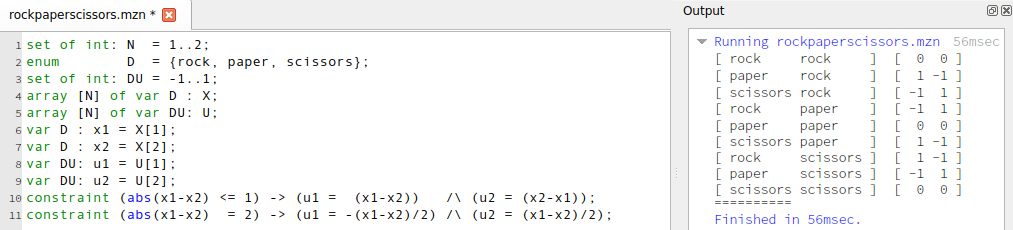
\includegraphics[width=1\linewidth]{images/mzn-rockpaperscissors.png}
    \end{minipage}}
    \caption{MiniZinc implementation of Rock-Paper-Scissors model}
    \label{fig:rockpaperscissors}
\end{figure}

\subsection{Solving Constraint Games}\label{sec:solvingconstraints}

To handle \hyperref[sec:rq]{RQ2}, we studied the method used to solve \constraintgames proposed by Nguyen \cite{nguyen:2015}, which aims to find strategies in Pure Nash Equilibrium by enumerating every \textit{strategy profile} $S$ and checking it using another search to find the \textit{best responses} $S'$ for each player. This method includes an additional database to store \textit{best responses} during the search, which will be compared in the future to save time. It also incorporates a set of counters for each \textit{player} to identify when the maximum possible \textit{best responses} are reached, leading to the termination of the search at the current level.  The Algorithm \ref{alg:enum} shows the highest level of this method. 

The aforementioned method was initially implemented in the Conga Solver by its author. We have replicated this method using an experimental solver, Python-CPSolver\git{https://github.com/GonzaloHernandez/python-cpsolver/blob/master/PythonCPSolver_Trail/propagators.py}, and we created another version using Chuffed+Gecode\git{https://github.com/GonzaloHernandez/equilibrium-chuffed}.

In order to enhance performance and design, we employed new constraint technologies that eliminate the need for additional memory storage and counters through the use of \textit{Clause Learning} (CL). We have proposed a novel method called \textit{Utility Guided Clause Learning} (UGCL).  This method aims to minimize the need for future \textit{strategy profile} checks by incorporating \textit{new} information, in the form of additional clauses $\vee_{j \ne i}(j \ne j^{new}) \vee (u_i \geqslant u_i^{new})$ into the main search, collected during the checking process. The Algorithm \ref{alg:ugcl} depicts our propagator used in this method.

The \textit{CDCL+UGCL Method} has been tested in Python-CPSolver, and we are currently working on implementing it in Chuffed, which already uses \textit{Conflict-Driven Clause Learning} (CDCL) \cite{stukey.2010}. This method was presented as a poster at OPTIMACON-24.

\subsection{Solving $\omega$-regular Games}\label{sec:solvingwregular}

To address \hyperref[sec:rq]{RQ1} we have studied and analyzed Zielonka's algorithm \cite{aggarwal:2023,ParysPaweł2019PGZA,vanDijk2018,ZielonkaWieslaw1998Igof}, an ad-hoc method for solving Parity games. The algorithm recursively decomposes the game into smaller subgames by identifying the highest priority and determining the sets of winning positions for each player, solving these subgames iteratively until the entire game is resolved. Although conceptually straightforward, Zielonka's algorithm is computationally intensive. Nevertheless, it remains a foundational tool in the analysis of parity games. We have implemented a version of this algorithm (see Algorithm~\ref{alg:zielonka}) using Python\git{https://github.com/GonzaloHernandez/constraint-games-draft/tree/master/paritygames} and have conducted an analysis of its behavior and the concept of \textit{attractors} \cite{huth2013,ArcucciRossella2017PPGa}.

An attractor in a parity game refers to a set of states that a particular player can control the game to reach, regardless of the opponent's moves \cite{ArcucciRossella2017PPGa,vanDijk2018}. The idea is that from any state within the attractor, the player can ensure that the game either stays within the attractor or eventually reaches a specific target set of states.  The computation of attractors occurs within the recursive process of Zielonka's algorithm. Figure \ref{fig:attractor} illustrates the set of vertices where Player $\bigcirc$ has control from vertex 5.

\begin{figure}[ht]
    \centering
    \noindent\fbox{\begin{minipage}{\dimexpr\textwidth-70\fboxsep-2\fboxrule\relax}
        \centering
        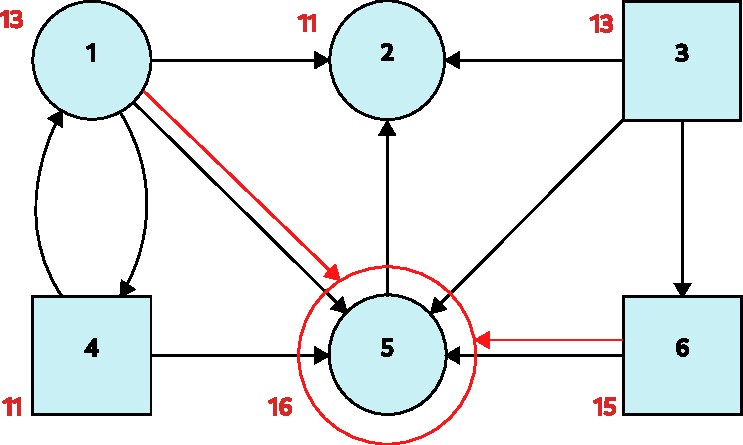
\includegraphics[width=0.7\linewidth]{images/attractor.pdf}
    \end{minipage}}
    \caption{$Attr_\bigcirc(5) = \{1,6\}$}
    \label{fig:attractor}
\end{figure}

To initially address \hyperref[sec:rq]{RQ1, RQ3}, we aim to explore the potential for mimicking the behavior of attractors within constraints.  An attractor is defined as $\textit{Attr}_i(Z) =  \{v \in V_i \mid E(v) \cap Z \ne \emptyset\} \cup \{v \in V_{-i} \mid E(v) \cap Z \subseteq Z\}$ for all $Z \subseteq V$ and $i \in N$ \cite{vanDijk2018}.

% -----------------------------------------------------------------------------

\section{Future Plan and Next Steps}\label{sec:plan}

We have completed several activities to advance the proposed research, addressing some aspects of \hyperref[sec:rq]{RQ2} and conducting initial work on \hyperref[sec:rq]{RQ1}. Table \ref{tab:planning} shows the planned timeline for completing each task in this research.

\begin{table}[H]\centering
    \newcommand{\y}{\cellcolor{black!50}}
    \newcommand{\n}{\cellcolor{white!100}}
    \newcolumntype{:}{!{\color{gray!20}\vrule}}
    \begin{tabular}{|r p{8.2cm}|l:l|l:l:l:l|l:l:l:l|l:l:l:l|l:l|}
        \hline
            & \textbf{Activities} 
            & \multicolumn{4}{c|}{\textbf{2023}} & \multicolumn{4}{c|}{\textbf{2024}} 
            & \multicolumn{4}{c|}{\textbf{2025}} & \multicolumn{4}{c|}{\textbf{2026}} \\
        \hline
            & Literature review 
            & \n & \n & \y & \y & \y & \n & \n & \n & \n & \n & \n & \n & \n & \n & \n & \n \\
            \arrayrulecolor{gray!20}\hline
        RQ1  & Encoding \wregulargames into \constraintgames
            & \n & \n & \n & \n & \n & \n & \y & \y & \y & \y & \y & \y & \n & \n & \n & \n \\
            \hline
        RQ2  & Solving Games with new constraint technologies
            & \n & \n & \n & \y & \y & \y & \n & \n & \n & \n & \y & \y & \y & \y & \n & \n \\
        \hline
        % RQ3  & Defining constraints and propagators for \wregulargames
        %     & \n & \n & \n & \n & \n & \n & \n & \n & \y & \y & \y & \y & \y & \y & \n & \n \\
        % \hline
        RQ3  & Evaluating \wregulargames Games framework
            & \n & \n & \n & \n & \n & \n & \n & \n & \n & \y & \y & \y & \y & \n & \n & \n \\
        \hline
            & Documentation
            & \n & \n & \n & \n & \n & \y & \n & \n & \n & \y & \n & \n & \y & \y & \y & \y \\
        \arrayrulecolor{black}\hline
    \end{tabular}
    \caption{Activity planning}
    \label{tab:planning}
\end{table}

% ------------------------------------------------------------------------
\newpage

\section*{Algorithms discussed in this document}
\setlength{\intextsep}{4pt}

\captionsetup[algorithm]{font=footnotesize}

\begin{algorithm}[H]
    \caption{Enumerate the strategy profiles in the CG-Enum-PNE \cite{nguyen:2015}}
    \footnotesize
    \begin{algorithmic}[1]
    \Procedure{ENUM}{domains $A$, int $i$}
        \If{$S$.propagate($A$)}
            \If{$i > n$}
                \State checkNash(tuple($A$), $n$)
            \Else
                \State $BR[i] \gets \emptyset$
                \State $cnt[i] \gets \prod_{j>i} |D_j|$
                \While{$A_i \neq \emptyset$}
                    \State choose $v \in A_i$
                    \State $B \gets A$
                    \State ENUM(($B$-$i$, $(B_i = \{v\})$), $i+1$)
                    \State $A_i \gets A_i - \{v\}$
                    \If{$cnt[i] \leq 0$}
                        \State checkEndOfTable($A$, $i$)
                        \State break
                    \EndIf
                \EndWhile
            \EndIf
        \EndIf
    \EndProcedure
    \end{algorithmic}
    \label{alg:enum}
\end{algorithm}

\begin{algorithm}[H]
    \caption{UGCL propagator}
    \footnotesize
    \begin{algorithmic}[1]
    \Function{UGCL-propagate}{solver $\Xi$, space $X,U$}
        \If{allAssigned($X$)}
            \For{$i \in N$}
                \State $\Xi' \leftarrow newSolver(\Gamma^c)$
                \State $clause \leftarrow []$
                \For{$(j \ne i) \in N$}
                    \State $\Xi'$.addConstraint( $\Xi'_{X_j} = X_j$ )
                    \State $clause \leftarrow clause \vee (\Xi_{X_j} \ne X_j)$
                \EndFor
                \State $\Xi'$.addConstraint( $\Xi'_{U_i} > U_i$ )
                % \State $\Xi'$.optimise( $\Xi'_{U_i}$ )
                \State $(X',U') \leftarrow \Xi'$.getSolution()
                \If{$(X',U') \ne \emptyset$}
                    \State $\Xi$.addConstraint( $clause \vee (\Xi_{U_i} \geqslant U'_i)$ )
                    \State \Return{false} 
                \EndIf
                \State $\Xi$.addConstraint( $clause \vee (\Xi_{U_i} \geqslant U_i)$ )
            \EndFor
        \EndIf
        \State \Return{true}
    \EndFunction
    \end{algorithmic}
    \label{alg:ugcl}
\end{algorithm}

\begin{algorithm}[H]
    \caption{Zielonka($G$) \cite{aggarwal:2023}}
    \footnotesize
    \begin{algorithmic}[1]
    \If{$V = \emptyset$}
        \State $(W_0, W_1) \gets (\emptyset, \emptyset)$
    \Else
        \State $m \gets \max\{\Omega(v) \mid v \in V\}$
        \State $q \gets m $ mod $ 2$
        \State $U \gets \{v \in V \mid \Omega(v) = m\}$
        \State $A \gets Attr_q(U)$
        \State $(W'_0, W'_1) \gets Zielonka(G \setminus A)$
        \If{$W'_{1-q} = \emptyset$}
            \State $(W_q, W_{1-q}) \gets (A \cup W'_q, \emptyset)$
        \Else
            \State $B \gets Attr_{1-q}(W'_{1-q})$
            \State $(W'_0, W'_1) \gets Zielonka(G \setminus B)$
            \State $(W_q, W_{1-q}) \gets (W'_q, W'_{1-q} \cup B)$
        \EndIf
    \EndIf
    \State \Return $(W_0, W_1)$
    \end{algorithmic}
    \label{alg:zielonka}
\end{algorithm}

% ------------------------------------------------------------------------

\newpage
\bibliographystyle{acm}
\bibliography{main}

% 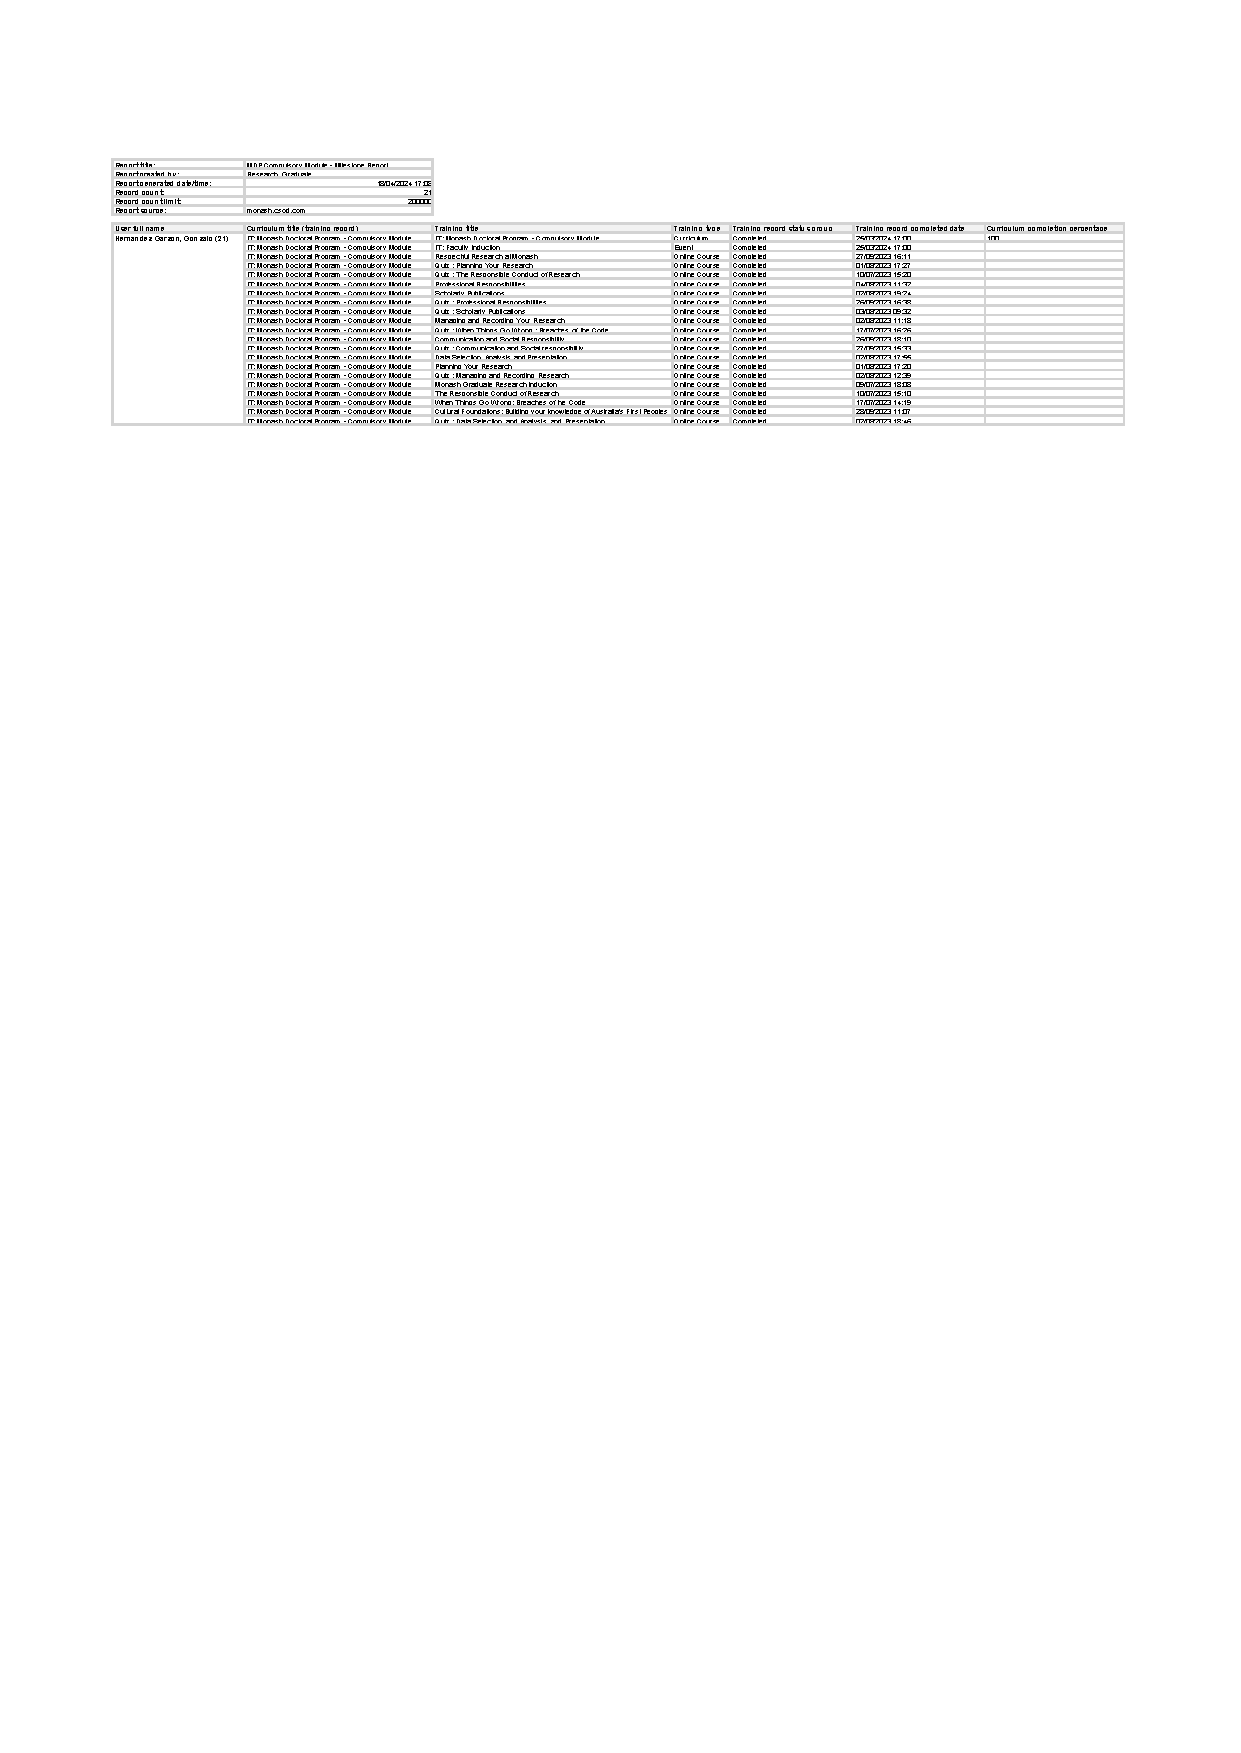
\includepdf[pages={1-1}]{attachments/MDP_Compulsory_Module-Milestone_Report.pdf} \label{appendix:a}
% 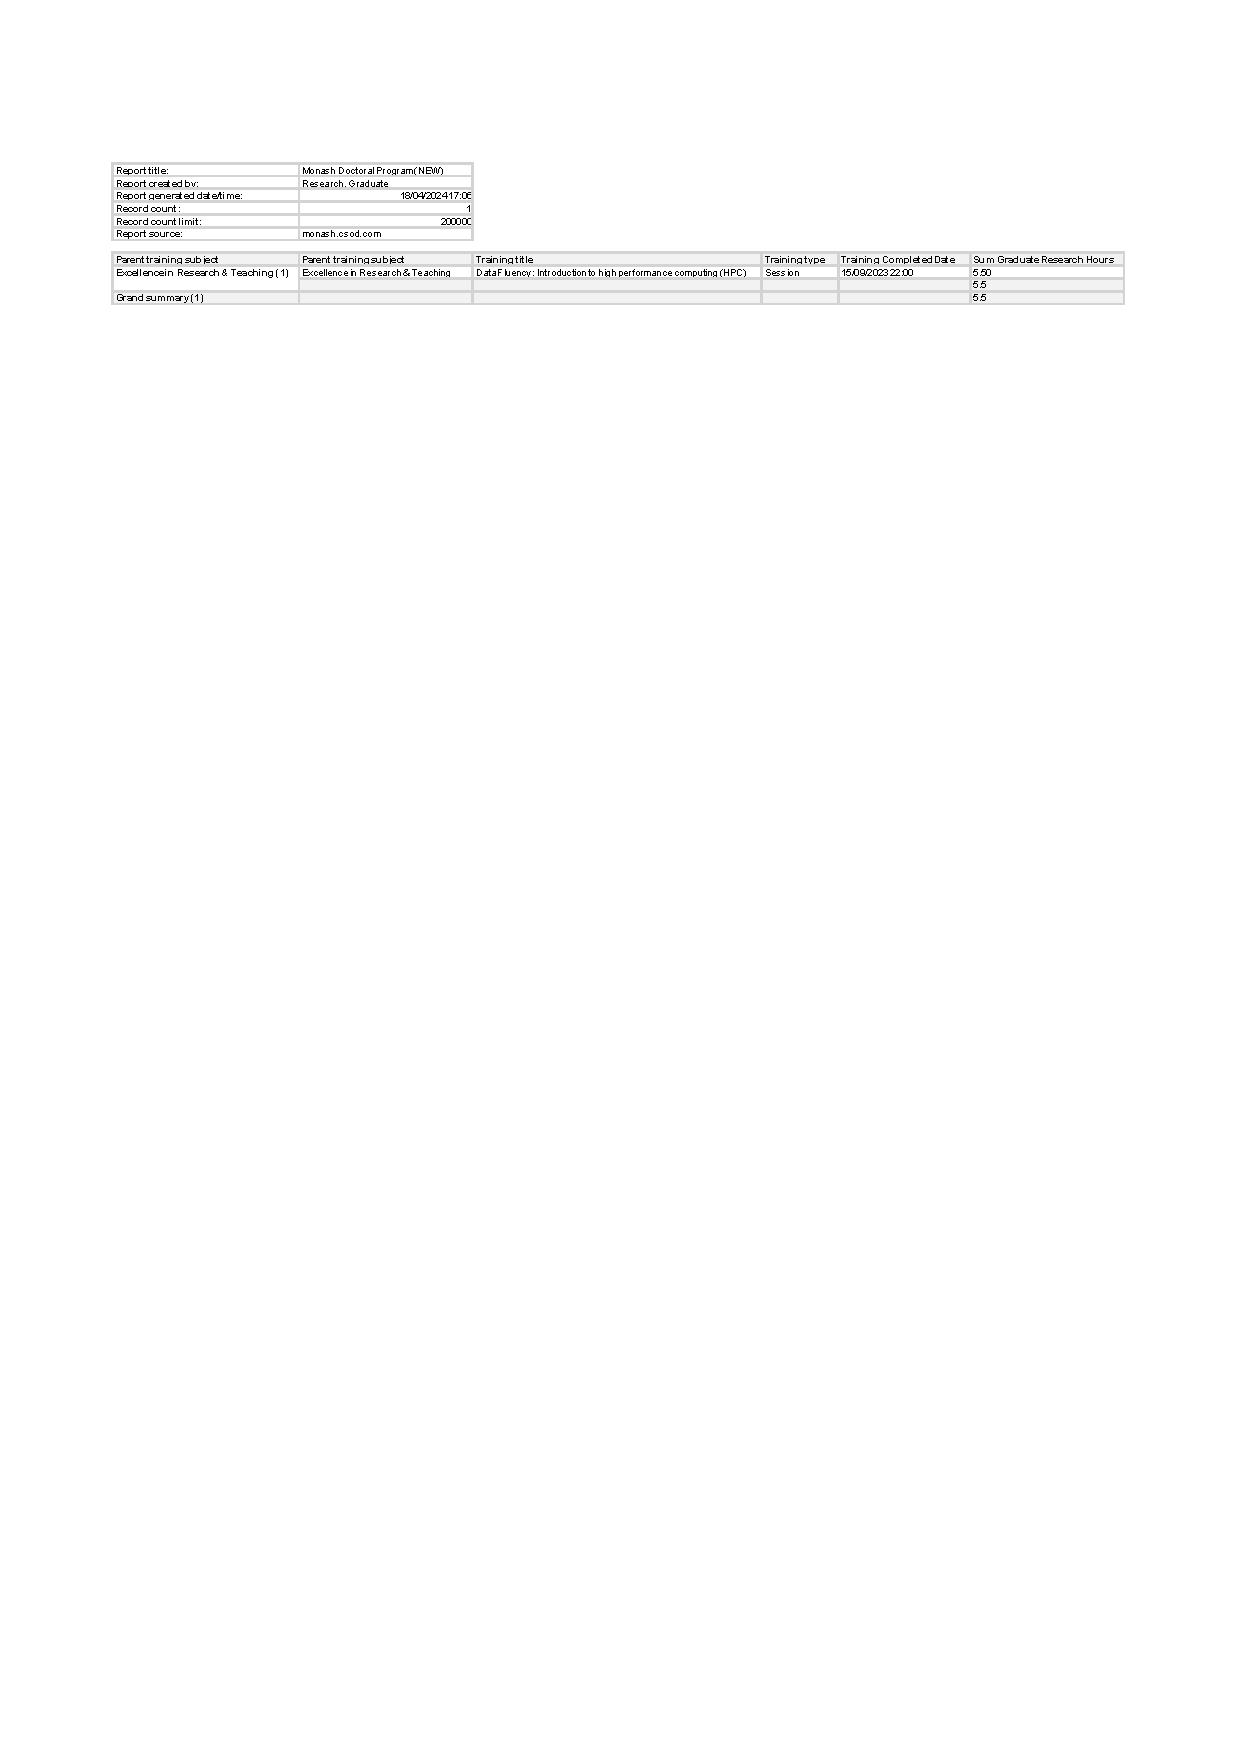
\includepdf[pages={1-1}]{attachments/Monash_Doctoral_Program_NEW.pdf} \label{appendix:b}

\end{document}